\subsection{IFIT2 Localisation in the Context of RSV pIBs} \label{subsec:IFIT2 Localisation in the Context of RSV pIBs}
\subsubsection{Single transfections}
%P Transfection Induces IFIT2A Signal but not IFIT2B Signal
Cell Line: 293T \newline
Treatment: hN and/or hP (EV – empty vector) \newline
Detecting magenta: endogenous human IFIT2 (A) \newline
Detecting cyan: N and/or P \newline

IFIT2 induction detected in hP and hP + hN conditions, suggesting that transfection of P induces IFIT2 expression (but this does not happen with IFIT1 or IFIT3 in the same cells).
About the different genomic regulation landscape… why does IFIT2 get induced but not other IFITs (within human genome which is well annotated)? 
Side note: No kinetochore microtubule staining (especially in first panel)

\begin{figure}
    \centering
    \includegraphics[width=1\linewidth]{10. Chapter 5/Figs/02. pIB/01. Single Transfection/01. 293t-ifit2a.pdf}
    \caption[ifit2a p transfection]{\textbf{ifit2a p transfection.} Nascent bovine IFIT1 in the context of bRSV infection has been observed to localise with the respect of IB in three distinct spaces. We observed it either concentrated inside the central point of the IB structure, while having reduced signal on the inner IB edge, compared to the cytoplasm (top and bottom panels), being excluded from the IB structure (3rd panel), or colocalising on the inner edge of the IB structure while having reduced signal in the middle of the structure compared to cytoplasm, or the edge staining (2nd panel).}
    \label{fig:ifit2a p transfection}
\end{figure}

Cell Line: 293T \newline
Treatment: hN and/or hP (EV – empty vector) \newline
Detecting magenta: endogenous human IFIT2 (B) \newline
Detecting cyan: N and/or P \newline

No detected IFIT2 induction in any of the conditions.
Side note: We can see kinetochore microtubule staining, especially in the first row.

\begin{figure}
    \centering
    \includegraphics[width=1\linewidth]{10. Chapter 5/Figs/02. pIB/01. Single Transfection/02. 293t-ifit2b.pdf}
    \caption[ifit2b p transfection]{\textbf{ifit2b p transfection.} Nascent bovine IFIT1 in the context of bRSV infection has been observed to localise with the respect of IB in three distinct spaces. We observed it either concentrated inside the central point of the IB structure, while having reduced signal on the inner IB edge, compared to the cytoplasm (top and bottom panels), being excluded from the IB structure (3rd panel), or colocalising on the inner edge of the IB structure while having reduced signal in the middle of the structure compared to cytoplasm, or the edge staining (2nd panel).}
    \label{fig:ifit2b p transfection}
\end{figure}

\subsubsection{pIBs}
%i2a 293t hnhp
Cell Line: 293T \newline
Treatment: hNhP \newline
Detecting magenta: endogenous human IFIT2 \newline
Detecting cyan: human pIB \newline

Nascent human IFIT2 strongly concentrates within the human RSV pseudo inclusion bodies.

\begin{figure}
    \begin{subfigure}{0.5\textwidth}
        \caption{}
        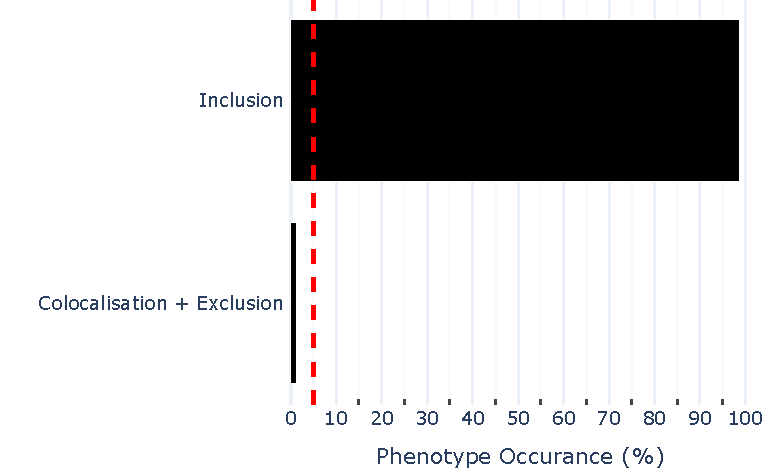
\includegraphics[width=1\linewidth]{10. Chapter 5/Figs/02. pIB/02. IFIT2A/01. bar_i2a_293t.pdf} 
    \end{subfigure}
    \begin{subfigure}{0.5\textwidth}
        \caption{}
        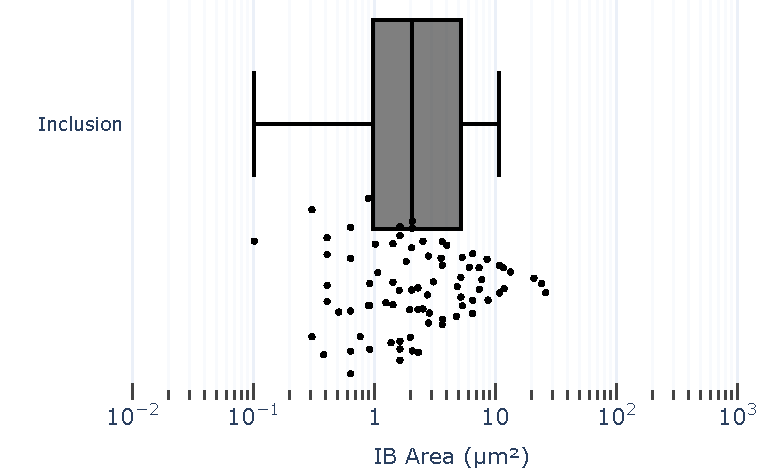
\includegraphics[width=1\linewidth]{10. Chapter 5/Figs/02. pIB/02. IFIT2A/02. box_i2a_293t.pdf}
    \end{subfigure}
    \begin{subfigure}{1\textwidth}
        \caption{}
        
\includegraphics[width=1\linewidth]{10. Chapter 5/Figs/00. placeholder.png} 
    \end{subfigure}
    \caption[i2a 293t hnhp]{\textbf{i2a 293t hnhp.} Nascent bovine IFIT1 in the context of bRSV infection has been observed to localise with the respect of IB in three distinct spaces. We observed it either concentrated inside the central point of the IB structure, while having reduced signal on the inner IB edge, compared to the cytoplasm (top and bottom panels), being excluded from the IB structure (3rd panel), or colocalising on the inner edge of the IB structure while having reduced signal in the middle of the structure compared to cytoplasm, or the edge staining (2nd panel).}
    \label{fig:i2a 293t hnhp}
\end{figure}

%i2a vero hnhp
Cell Line: VERO \newline
Treatment: hNhP \newline
Detecting magenta: endogenous monkey IFIT2 \newline
Detecting cyan: human pIB \newline

Endogenous monkey IFIT2 colocalises with the pIB structure (probably like an inclusion), as well as with the pIB filamentous network.

\begin{figure}
    \begin{subfigure}{0.5\textwidth}
        \caption{}
        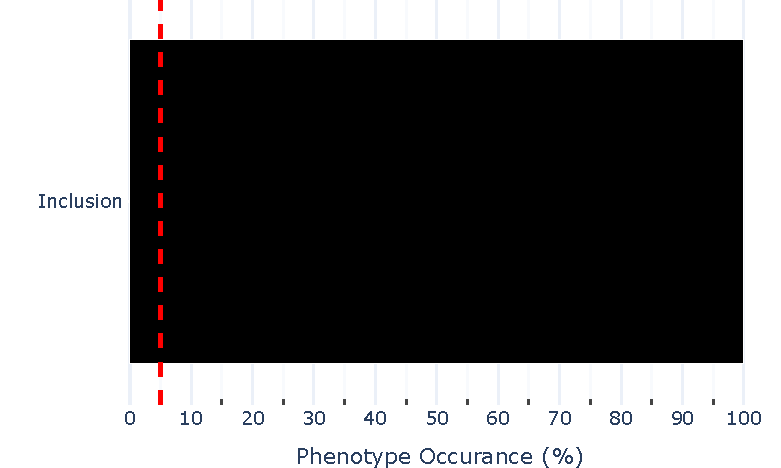
\includegraphics[width=1\linewidth]{10. Chapter 5/Figs/02. pIB/02. IFIT2A/04. bar_i2a_vero_hnhp.pdf} 
    \end{subfigure}
    \begin{subfigure}{0.5\textwidth}
        \caption{}
        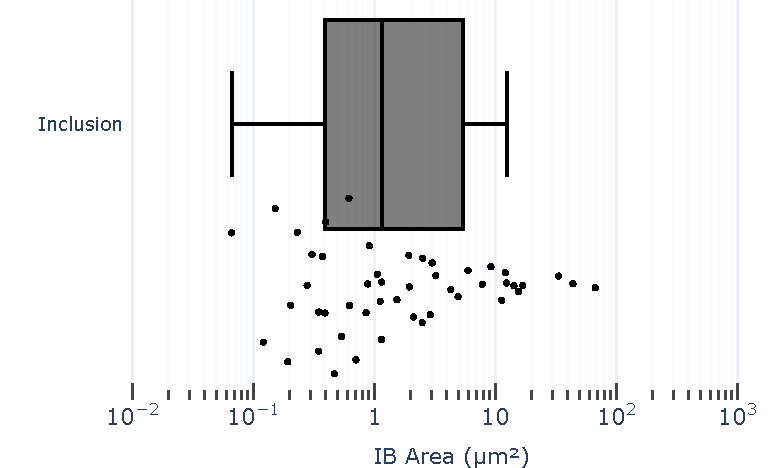
\includegraphics[width=1\linewidth]{10. Chapter 5/Figs/02. pIB/02. IFIT2A/05. box_i2a_vero_hnhp.pdf}
    \end{subfigure}
    \begin{subfigure}{1\textwidth}
        \caption{}
        
\includegraphics[width=1\linewidth]{10. Chapter 5/Figs/00. placeholder.png} 
    \end{subfigure}
    \caption[i2a vero hnhp]{\textbf{i2a vero hnhp.} Nascent bovine IFIT1 in the context of bRSV infection has been observed to localise with the respect of IB in three distinct spaces. We observed it either concentrated inside the central point of the IB structure, while having reduced signal on the inner IB edge, compared to the cytoplasm (top and bottom panels), being excluded from the IB structure (3rd panel), or colocalising on the inner edge of the IB structure while having reduced signal in the middle of the structure compared to cytoplasm, or the edge staining (2nd panel).}
    \label{fig:i2a vero hnhp}
\end{figure}


\begin{figure}
    \begin{subfigure}{0.5\textwidth}
        \caption{}
        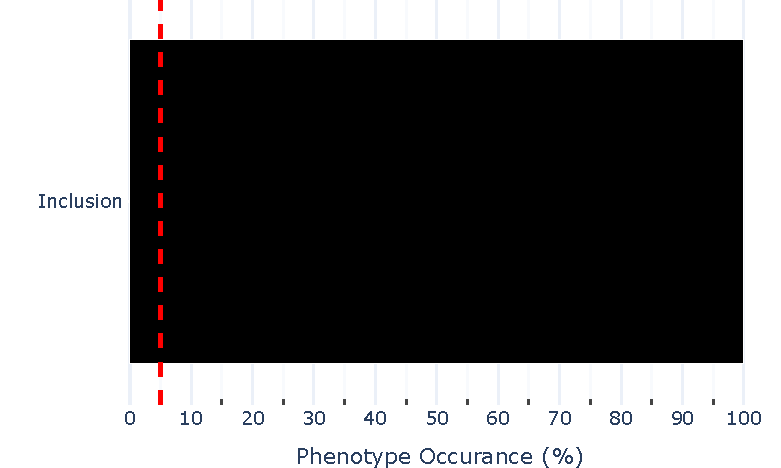
\includegraphics[width=1\linewidth]{10. Chapter 5/Figs/02. pIB/02. IFIT2A/07. bar_i2a_vero_bnbp.pdf} 
    \end{subfigure}
    \begin{subfigure}{0.5\textwidth}
        \caption{}
        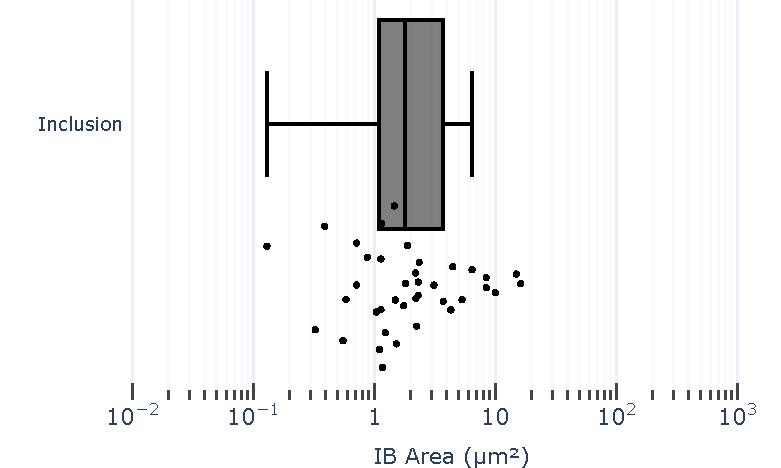
\includegraphics[width=1\linewidth]{10. Chapter 5/Figs/02. pIB/02. IFIT2A/08. box_i2a_vero_bnbp.pdf}
    \end{subfigure}
    \begin{subfigure}{1\textwidth}
        \caption{}
        
\includegraphics[width=1\linewidth]{10. Chapter 5/Figs/00. placeholder.png} 
    \end{subfigure}
    \caption[i2a vero bnbp]{\textbf{i2a vero bnbp.} Nascent bovine IFIT1 in the context of bRSV infection has been observed to localise with the respect of IB in three distinct spaces. We observed it either concentrated inside the central point of the IB structure, while having reduced signal on the inner IB edge, compared to the cytoplasm (top and bottom panels), being excluded from the IB structure (3rd panel), or colocalising on the inner edge of the IB structure while having reduced signal in the middle of the structure compared to cytoplasm, or the edge staining (2nd panel).}
    \label{fig:i2a vero bnbp}
\end{figure}

%i2b vero hnhp
Cell Line: VERO \newline
Treatment: hNhP \newline
Detecting magenta: endogenous monkey IFIT2 \newline
Detecting cyan: human pIB \newline

Nascent monkey IFIT2 is completely excluded from the human RSV pseudo-IBs and the pIB filamentous network.

\begin{figure}
    \begin{subfigure}{0.5\textwidth}
        \caption{}
        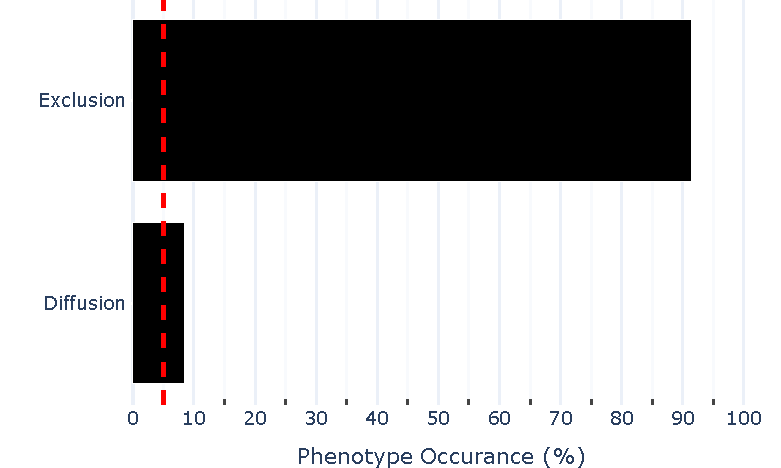
\includegraphics[width=1\linewidth]{10. Chapter 5/Figs/02. pIB/03. IFIT2B/01. bar_i2b_hnhp.pdf} 
    \end{subfigure}
    \begin{subfigure}{0.5\textwidth}
        \caption{}
        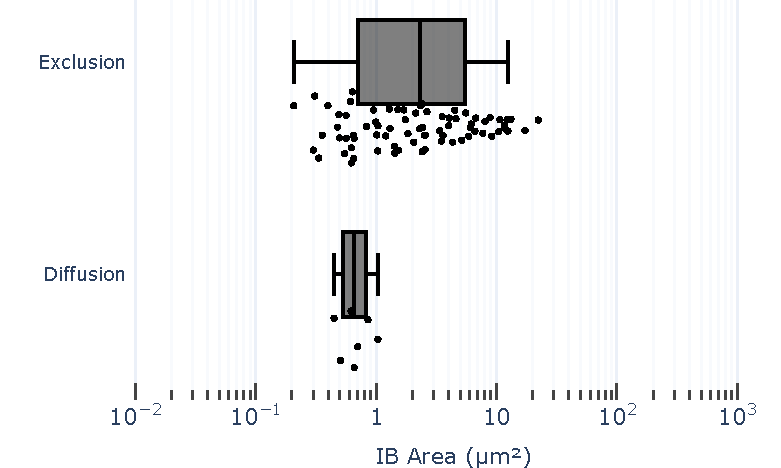
\includegraphics[width=1\linewidth]{10. Chapter 5/Figs/02. pIB/03. IFIT2B/02. box_i2b_hnhp.pdf}
    \end{subfigure}
    \begin{subfigure}{1\textwidth}
        \caption{}
        
\includegraphics[width=1\linewidth]{10. Chapter 5/Figs/00. placeholder.png} 
    \end{subfigure}
    \caption[i2b vero hnhp]{\textbf{i2b vero hnhp.} Nascent bovine IFIT1 in the context of bRSV infection has been observed to localise with the respect of IB in three distinct spaces. We observed it either concentrated inside the central point of the IB structure, while having reduced signal on the inner IB edge, compared to the cytoplasm (top and bottom panels), being excluded from the IB structure (3rd panel), or colocalising on the inner edge of the IB structure while having reduced signal in the middle of the structure compared to cytoplasm, or the edge staining (2nd panel).}
    \label{fig:i2b vero hnhp}
\end{figure}

\subsubsection{Summary} \label{Summary-i2-pib}
Both endogenous human and monkey IFIT2 forms inclusions inside human RSV pseudo-IBs. Monkey IFIT2 also colocalises to the pIB filamentous network (this structure was not observed in the human experiment). The identical staining can be observed in monkey cells with overexpressed human IFIT2-FLAG.

Endogenous monkey IFIT2 is excluded from human pIB and the pIB associated filamentous network. Overexpressed human IFIT2-FLAG is detected by the antibody and shows inclusions inside the human pIB structures, which is consistent to data from IFIT2A staining and FLAG staining of IFIT2-FLAG overexpressed samples. Interestingly, IFIT2B antibody shows exclusion from the pIB filamentous network, which was colocalised by IFIT2A and FLAG antibodies.